\documentclass[12pt]{article}

\usepackage[left=2cm, right=2cm, top=2cm, bottom=2cm]{geometry}
\pagenumbering{arabic}
\usepackage{footnote}
\usepackage{graphicx}
\usepackage{amsmath}
\usepackage[font={footnotesize}]{caption}
\usepackage{natbib}
\usepackage{wrapfig}
\usepackage{color}
\usepackage{setspace}
\usepackage{url}
\usepackage{fancyhdr}
\usepackage{enumitem}

\setlength{\bibsep}{1pt}

\pagestyle{fancyplain}
\lfoot{\small Brooke Simmons}
\rfoot{\small Shane Proposal ID ????}
\lhead{}
\rhead{}

\renewcommand{\headrulewidth}{0pt}
\renewcommand{\refname}{\normalfont\selectfont\normalsize\bf References}

\def\lesssim{\mathrel{\hbox{\rlap{\hbox{\lower3pt\hbox{$\sim$}}}\hbox{\raise2pt\hbox{$<$}}}}}

\begin{document}

\noindent \emph{Shane Proposal ID ???? (2018A), Kast Double-Beam Spectrograph, ? nights} \\
\noindent \emph{PI: Brooke Simmons - Title: {\bf Bulgeless quasars; constraining secular inflows with measurements of outflows}} 
\vspace{0.5em}

\noindent {\bf Scientific Justification}
\vspace{0.25em}

Understanding the co-evolution of galaxies and their central supermassive black holes (SMBHs) is integral to modern astrophysics. Determining the physical processes which drive the growth of the main structure of a galaxy and which are tightly coupled to those which govern SMBH growth is a key goal of current observational programs. An increasing body of evidence shows that galaxy growth is mainly dependent on `secular processes' rather than by mergers; Kaviraj et al.$^{[1]}$, for example, have shown that only $27\%$ of star formation is triggered by major or minor mergers. Therefore if galaxy growth is dominated by secular processes, then it follows that these processes also dominate SMBH growth.
\vspace{0.25em}

This proposal aims to estimate the amount of material driven to the central regions of a galaxy through secular processes and the amount of energy injected back into the galaxy by active galactic nucleus (AGN) feedback in galaxies whose evolution is dominated by secular processes. We shall do so by measuring the rate of mass loss in AGN outflows from the central region of disk-dominated galaxies. The outflow measurements are enabled with narrow-band imaging of the nearby galaxies in our sample; by combining this measurement with existing data constraining the black hole accretion rate, this will provide a limit on the total inflow rate to the centre of the galaxy. The lack of significant bulge (or pseudo-bulge) in these disk-dominated systems (see Figure 1) indicates a dynamical history which is free of significant mergers therefore we can therefore assume that any inflow is driven solely by secular processes. Much of this inflowing material into the central regions of the galaxy will not be accreted by the black hole, but rather will form an outflow. Such outflows are common in AGN and can be very significant. Bae et al.$^{[2]}$ show that the flux of material in outflows in twenty nearby AGN is an order of magnitude larger than the rate of accretion for the black hole.
\vspace{0.25em}

By using a sample of galaxies where we can be sure that secular processes dominate we can, for the first time, understand what the limits to merger-free black hole growth are. We will utilise a well-studied sample of disk-dominated galaxies with unobscured AGN. The sample comprises galaxies in the SDSS spectroscopic sample cross-matched with X-ray survey data to identify AGN$^{[3,4]}$. The disk-dominated morphologies were identified by expert review, either of the SDSS imaging, shown in Figure 1, or via an ongoing HST snapshot survey (see example in Figure 2) with broadband imaging using ACS WFC (Prop. ID 14606, PI: Simmons). 
\vspace{0.25em}

The spectra of these systems were kinematically fitted, each with two components identified for the \textsc{[oiii]} $5007\rm{\AA}$ emission line. The main emission line is identified from the expected wavelength relative to the emission lines in the rest of the spectrum, and the blueshifted component is attributed to the outflow. Although we know from the spectra that there is \emph{some} outflowing material either within the fiber or along the slit, these do not permit a full measurement of the energy deposited into the galaxy via outflows. We thus propose to observe these outflows using narrow band imaging centred on the blueshifted component of the \textsc{[oiii]} $5007\rm{\AA}$ emission line. This will allow for measurements of the outflow luminosity which can be used to calculate a gas mass in the outflow following the method outlined in Carniani et al. (2015)$^{[6]}$:
\begin{equation}
M_{\rm{gas}} = 0.8 \times 10^8~M_{\odot} \left( \frac{C}{10^{[O/H] - [O/H]_{\odot}}} \right) \left( \frac{L_[OIII]}{10^{44}~\rm{erg}~\rm{s}^{-1}} \right) \left( \frac{n_e}{500~\rm{cm}^{-3}} \right)^{-1}
\end{equation}

where $n_e$ is the electron density, $[O/H] - [O/H]_{\odot}$ is the metallicity relative to solar, and $C = <n_e>^2 / <n_e^2>$. Here $<n_e>^2$ is the volume averaged electron density squared and $<n_e^2>$ is the volume averaged squared electron density. This method requires some simplifying assumptions on the nature of the outflowing gas, particularly on the temperature and density of the gas, however these caveats affect all such measurements in the literature which we intend to use as part of a control sample. 
\vspace{0.25em}

Combining this measurement of the gas mass with the velocity of the outflow measured from the spectra and the spatial extent of the outflow will allow us to measure the mass loss rate due to the outflow. This measurement will hence allow us to compute the amount of energy involved in AGN feedback in pure disk systems, as well as to derive a limit on the inflow rate powered by secular processes in each of these systems. 
\vspace{0.25em}
 
The results for this particular disk-dominated sample will be compared with the more typical systems of Bae et al.,$^{[2]}$ which have morphologies indicative of an evolutionary history containing (at least) minor mergers. If the inflow rate for the two sets of galaxies is similar, the obvious conclusion is that secular processes fuel black hole growth and outflows regardless of morphology. This result would support work by Simmons et al.$^{[3]}$ and Simmons, Smethurst \& Lintott$^{[4]}$ who find a relation between black hole and total stellar mass which is shared between both disk-dominated and bulge-dominated systems (see Figure 3). On the other hand, if the inflow rates derived for these disk-dominated systems are significantly less than that in the control systems of Bae et al.,$^{[2]}$ then for the first time we will have properly constrained the relative contributions to present-day black hole growth from secular processes and mergers. These observations are thus likely to produce significant insight to a major problem in the study of galaxy evolution. 
\vspace{1.5em}


\noindent {\bf Figures and References}
\vspace{0.5em}


\noindent
$[1]$ Kaviraj et al. 2013, MNRAS, 429, 40
\\
$[2]$ Bae et al. 2017, ApJ, 837, 91
\\
$[3]$ Simmons et al. 2013, MNRAS, 429, 2199 
\\
$[4]$ Simmons, Smethurst \& Lintott (submitted to MNRAS)
\\
$[5]$ Haring \& Rix, 2004, ApJ, 604, 89
\\
$[6]$ Carniani et al. 2015, A\&A, 580, 102

\begin{figure}[h]
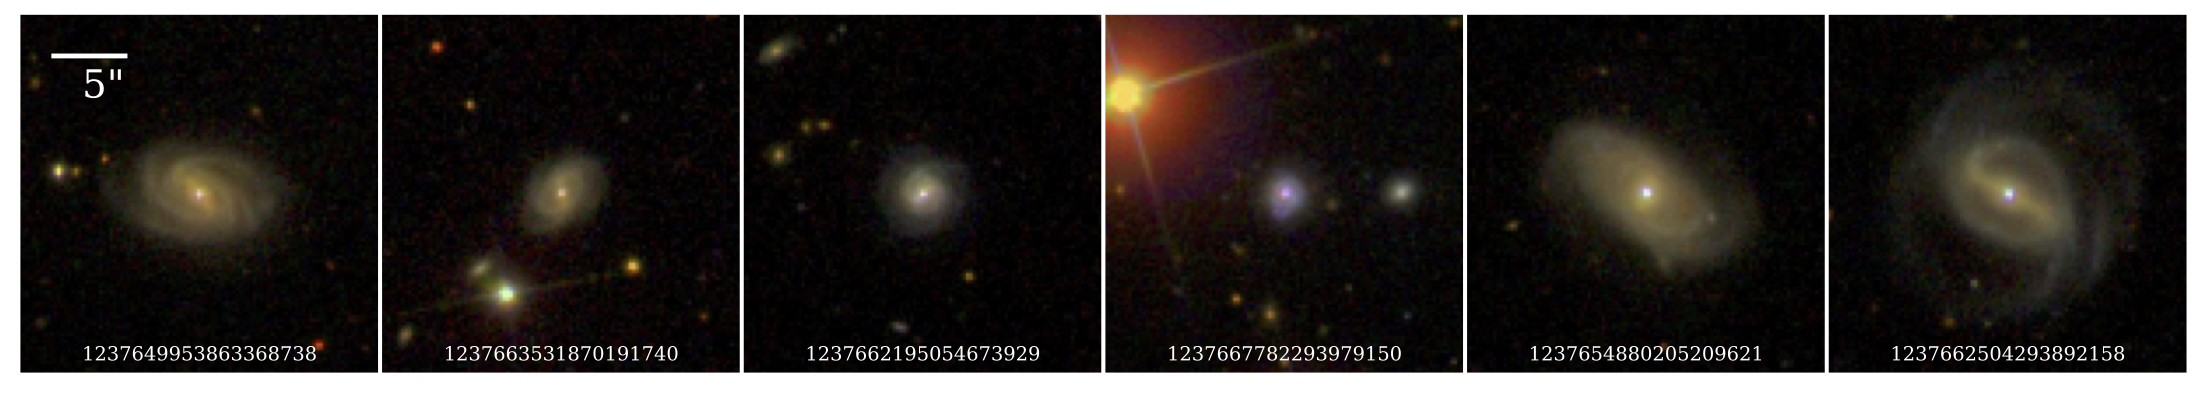
\includegraphics[width=\textwidth]{mosaic_6_2017B_obs.png}
\caption{SDSS ugriz postage stamp images of the six disk-dominated galaxies in this proposal sample. In all the images, the bright point source of the AGN is clearly visible.}
\end{figure}

\begin{figure} [h]
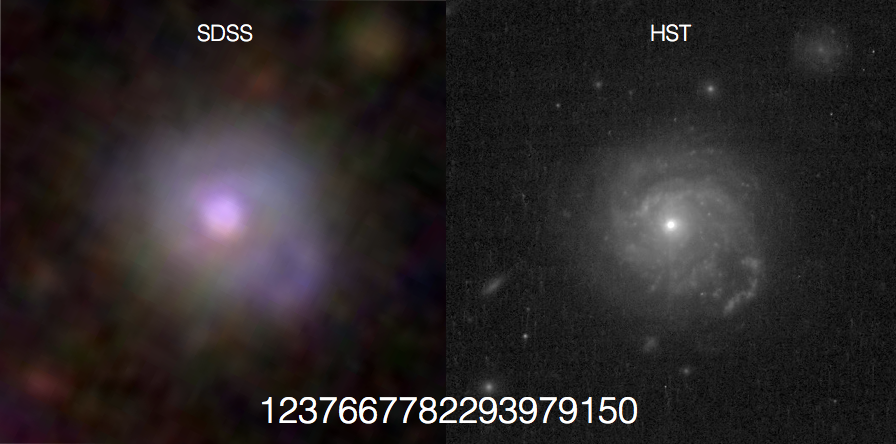
\includegraphics[width=0.5\textwidth]{fig3.png} \\
\caption{SDSS ugriz postage stamp image of galaxy 1237667782293979150 (left) in comparison with HST ADS WHT image (right), which confirms its disk-dominated morphology.}
\end{figure}

\begin{figure} [h]
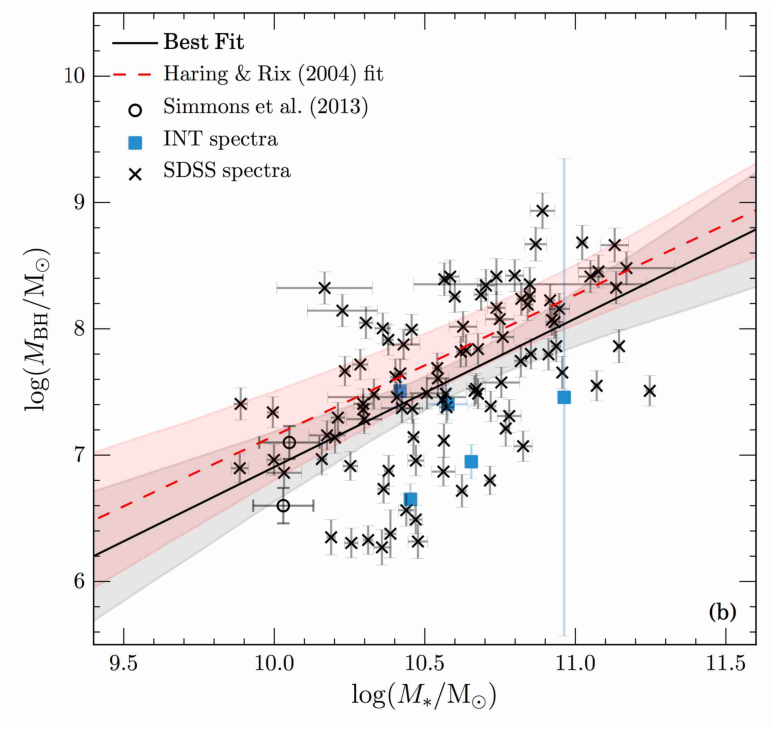
\includegraphics[width=0.5\textwidth]{fig2_r.pdf} \\
\caption{Black hole mass versus total stellar mass$^{[4]}$ derived from SDSS spectra (black crosses) and from INT spectra (blue squares; semester 2014A) for our entire disk-dominated sample. The six galaxies in this proposal are highlighted by the green circles. The best-fit line to the disk-dominated sample is shown in black (solid line), with the relation for early-types from Häring \& Rix$^{[5]}$ shown in red (dashed line). The relations are consistent for populations of disk-dominated and early-type galaxies, suggesting secular processes must fuel black hole growth regardless of morphology.}
\end{figure}


\noindent {\bf Supplementary Observations Required from Other Observatories}
\\
No additional observations are required from other observatories.

\noindent {\bf Technical Remarks}
\\
This proposal is informed by conversation with UCO/Lick support astronomers and telescope operators. The availability of a variety of narrow-band filters makes Lick an optimal facility for imaging the outflows of relatively nearby AGN. We had originally considered applying for time on the Nickel, but conversations with Mt. Hamilton staff encouraged us to consider using Kast as an imager with the narrow-band filters currently housed at the 3-m. However, we are very open to further discussions if some other setup would make best use of the facilities.

This is a study of six disk-dominated AGN host galaxies using narrow-band imaging to observe outflows in \textsc{[OIII]} $5007\rm{\AA}$ with the ACAM on the WHT. Narrow-band imaging will allow the luminosity and spatial extent of the outflow to be determined, so that the gas mass in the outflow and therefore the outflow rate can be determined. The six galaxies are spread across the sky such that the best time for observations is during dark skies in January.
\vspace{0.25em}

From the SDSS spectra, we have the observed  wavelength of the narrow \textsc{[oiii]} $5007\rm{\AA}$ component for all 101 galaxies is our disk-dominated AGN host sample (shown in Figure 3). This gives redshifted wavelengths in the range of $5165-6231~\rm{\AA}$ for the full sample. This allows us to choose from the ING narrow-band filter database the filter which results in the highest transmission at the observed wavelength. Of all the galaxies in our disk-dominated sample, 6 have redshifted \textsc{[oiii]} $5007\rm{\AA}$ emission lines which are observable in a filter with a FWHM $\leq15\rm{\AA}$. We have chosen to use such narrow filters (rather than those in the database with FWHM $\sim450\rm{\AA}$) in order to isolate the \textsc{[oiii]} $5007\rm{\AA}$ emission and reduce contamination from nearby \textsc{[feii]}, \textsc{[ni]} and H$\beta$ emission. 
\vspace{0.25em}

Similarly, we have chosen appropriate narrow-band filters to observe the continuum of each galaxy away from the observed emission lines in the spectra. Continuum measurements are required to isolate the flux purely in \textsc{[oiii]} $5007\rm{\AA}$ emission, from the continuum at that wavelength. The \textsc{[oiii]} $5007\rm{\AA}$ emission of the outflow will be isolated from the centrally concentrated \textsc{[oiii]} $5007\rm{\AA}$ emission of the nucleus spatially in the resulting narrow-band images. 
\vspace{0.25em}

Given the energy per \textsc{[oiii]} $5007\rm{\AA}$ photon, the throughput of each of the chosen narrow-band filters and assuming negligible sky background noise on dark sky nights  with respect to the read noise of the \textsc{auxcam} chips, we calculated the exposure times required to reach a S/N $\sim 3$ per pixel for both the \textsc{[oiii]} $5007\rm{\AA}$ and continuum for each source. Given this requirement the maximum combined on-source time is $250.3$~minutes ($4.2$ hours), assuming a seeing of $1"$ and an airmass of $1.5$. The total combined on-source time is $859.1$ minutes.  
\vspace{0.25em}

Using this information combined with the overhead estimates from the ACAM Total Observing Time Estimator and considering the average weather downtime of $34\%$ in January, we calculate that we can observe all 6 targets in 2.27 nights of dark skies in January of the 2017B semester, therefore we have requested 3 dark sky nights of observing time. Observations will also be possible split across 2 dark sky nights, with 1 night in August-September and 2 in January.

{\bf Path to Science}
\\
Given the uniqueness of these sources as AGN hosted in disk-dominated galaxies yet with clear signs of outflows, these targets are publishable in comparison with more ``typical'' examples of AGN outflows. Following reduction of the data, we will use standard techniques to measure luminosity and subtract the continuum in order to use the method described above to estimate the mass outflowing and place limits on inflowing mass. The next steps after the publication of the first paper depend somewhat on the results; it may be that the diversity of morphologies and luminosities lead us to propose for additional observations of the sample, but even should this not be the case there is a clear path to at least 1 publication with this data set.

{\bf Status of Previously Approved 3-m Programs}
\\
This is a sub-sample from a larger sample observed over the past several semesters at Lick. These AGN hosted in disk-dominated galaxies are a rich sample of interesting sources; the primary driver for the science was the measurement of black hole masses for comparison to bulge- and galaxy stellar masses, as part of an ongoing program including multi-wavelength SDSS and \emph{HST} imaging. The secondary purpose for observing these with the Shane/KAST setup is to investigate the star formation properties of these disk galaxies. Both programs are ongoing; the \emph{HST} program has just completed, the Lick data is being reduced as it comes in (we still have further nights scheduled in 2017B) and a paper is in progress. The outflows in the sample were a serendipitous discovery while measuring black hole masses, and led to this proposal. 

{\bf Backup Observing Program}
\\
We can observe the same targets even in poor seeing, as the narrow wavelength bands mean we are less likely to be contaminated by the main AGN [OIII] luminosity even if the PSF extends over more pixels than is ideal. If there are wind restrictions or similar, we can focus on the subset of targets that are within the restricted cone. If there is an issue with the filter wheel or the non-standard setup we have proposed, we can observe our targets in the more standard spectrographic setup, with a slit pattern designed to approximate 2-D coverage of the targets. While this is not ideal from a data reduction standpoint, its availability as a backup program means we are robust to many potential failure modes. 

{\bf Target Source List}
\\

{\bf Abstract}

\end{document}
